\chapter{Implementation Details}
    In this section I will go into detail about monitoring techniques, communication between various components and how the system was
    implemented.

    \section{Activity Monitoring}

    Monitoring activity from a minifilter driver is the most reliable way of monitoring and blocking potentially malicious Linux applications.
    Unlike a user-mode hooking framework approach, using a minifilter driver provides mechanisms of monitoring that cannot be bypassed or tampered
    with by the monitored processes, making it a very reliable and secure approach.

    \subsection{Process Monitoring}
        Process monitoring refers to getting synchronous notifications on both process creation and process termination in order to keep track
        of the currently active processes and process hierarchy.

        \paragraph{}
        In order to receive these notifications, the driver must register a callback with PsSetCreateProcessNotifyRoutineEx2. This callback will
        be called for both win32 processes and pico processes. To identify a WSL process, the driver must call ZwQueryInformationProcess with
        SubsystemInformationTypeWSL information type on the process' handle and check that the subsystem type is SubsystemInformationTypeWSL.

        \paragraph{}
        All monitored processes are stored in a structure named "Process Collector". We monitor only Linux processes and Windows processes that
        have their parent process in the collector. The second condition is needed because we have to monitor Windows processes that are started
        by Linux processes.

        For each monitored process we hold an object called Process, which is allocated from a paged memory lookaside list, in order to
        optimize allocations. A lookaside list is a cache of free memory blocks. Whenever we allocate an object from a lookaside list, if
        an empty block is available, we pop the empty block from the list and use it, otherwise we allocate from the paged pool. Whenever we
        free an object allocated from a lookaside list, we push it into the cache if it is not full. Otherwise we actually free the memory block.

        Since many processes are started and terminate throught the run time of the system, using lookaside lists for our "Process" objects
        turned out to be an important optimization.
        
        \paragraph{}
        The thread safety of the lookaside list's push and pop operations is given by the usage of InterlockedPushEntrySList and
        InterlockedPopEntrySList Windows APIs, that use SLIST\textunderscore ENTRY nodes, which are actually nodes in a singly linked list.

        \subsection{File System Activity Monitoring}
        File system activity monitoring refers to monitoring the disk I/O operations a process does and identifying relevant events such as
        rename, delete, etc. These events that play a vital role in identifying potentially malicious behavior (i.e dropping an executable in
        C:\textbackslash Windows\textbackslash System32).
        
        Monitoring file system activity can be easily done with a minifilter driver by
        registering "pre" and "post" callbacks for various operations (i.e. IRP\textunderscore MJ\textunderscore CREATE).

    Example callbacks registration:

    \begin{Verbatim}[fontsize=\small, commandchars=\\\{\}]
\textcolor{blue}{constexpr} \textcolor{cyan}{FLT_OPERATION_REGISTRATION} OperationRegistration[] =
\{
    \{
        \textcolor{magenta}{IRP_MJ_CREATE},
        0,
        PreCreateCallback,
        PostCreateCallback
    \},
    ...
    
    \{ \textcolor{magenta}{IRP_MJ_OPERATION_END}, \}
\};
    \end{Verbatim}

    \paragraph{}
    After registering the callbacks above, for every IRP\textunderscore MJ\textunderscore CREATE IRP (I/O request packet), "PreCreateCallback"
    will be called before actually doing the operation, giving us the opportunity to skip the post callback call if needed, and
    "PostCreateCallback" will be called after the operation was completed, giving us information about the completion status, used file object,
    etc.

    An IRP is a partially opaque and self contained structure that represents an I/O operation and holds all of the information needed by
    a driver to handle that I/O request. The I/O manager creates an IRP in memory to represent an I/O operation, passing a pointer to the
    IRP to the correct driver and disposing of the packet when the I/O operation is complete\cite{WindowsInternals62}.

    \paragraph{}
    In order to identify the requestor of the IRP we call FltGetRequestorProcessId, which gives us the PID of the process. The RequestorMode
    field can be either KernelMode or UserMode, telling us whether the IRP was issued by the kernel or not. Traditionally, most AV-solutions
    would skip KernelMode IRPs, as they would not be important.
    
    This was one of the issues that came along with WSL, as Linux processes, not knowing of the Windows kernel, can't issue IRPs by their own.
    Instead, the pico provider (lxcore.sys) issues them, therefore the IRPs have  RequestorMode equal to KernelMode. However, the requestor PID
    is that of the actual process that started the I/O operation, therefore the IRP filtering algorithm would filter KernelMode IRPs too, if
    and only if the requestor PID is different than system process PID.

    \pagebreak

    \section{Communication}
        
        Two communication channels were implemented for this application:
        \begin{enumerate}
            \item wslflt.sys to wslcore.dll
            \item wslamss.exe to WSL Anti-Malware.exe
        \end{enumerate}

        \paragraph{}
        The first communication channel is designed to provide a user-mode component with control over the driver while also giving the driver
        the ability to notify a user-mode component about certain events (i.e. detection).
        
        Communication between the driver and the dll used for integration is implemented using Windows Filter Ports. This is a minifilter
        specific communication technology which enables two-way communication between a minifiter driver, acting as a server, and a user-mode
        application, acting as a client.

        \paragraph{}
        The second communication channel has the purpose of connecting the .NET service which integrates the SDK to the GUI application and is
        a two-way, RPC like, net.tcp protocol channel.

        The server endpoint is located in the .NET service which integrated the SDK, while the client service is located in the GUI application.
        Both endpoints have similar architecture, where requests from the other side are implemented as .NET events, and requests towards the other
        side are done through an service contract interface.

        For now, the service provides only one type of notification, which is the process detected notification, which is listened to by the GUI
        application in order to send a toast notification to the system, informing the user of the detection.
        The requests that the service can resolve are:
        
        \begin{itemize}
            \item start monitoring
            \item stop monitoring
            \item get detection history
            \item query current settings
        \end{itemize}

    \section{Detection Flow}
        Based on the communication model presented above, I will present the flow of a detection, starting from the wslflt.sys kernel driver
        to the GUI Application and toast notification.
        
        \paragraph{}
        The kernel driver is responsible for issuing the detection and stopping the malicious process. After doing this the user mode system
        service is informed through the filter port. The system service relays the detection information to the GUI application through the WCF
        endpoint. Finally, a toast notification is displayed in order to inform the user of the detection.

        \begin{figure}[H]
            \centering
            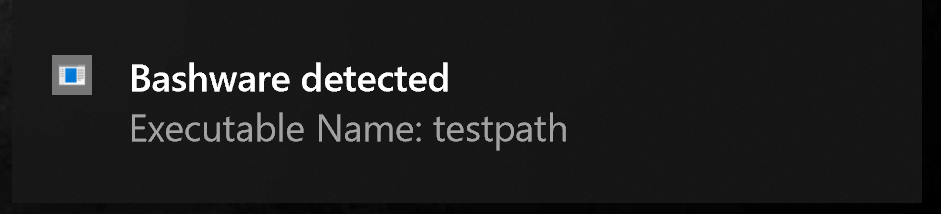
\includegraphics[width=300px, keepaspectratio]{img/detection.png}
            \caption{Detection Notification}
            \label{fig:detection}
        \end{figure}

        Clicking the notifications brings the application to front and selects the detections tab, so that the user can see more information
        about the detection.


    \section{C++ Memory Allocation Framework in the Kernel}
        Allocating memory in the kernel is done via the ExAllocatePool API family (i.e. ExAllocatePoolWithQuotaTag, ExAllocatePool,
        ExAllocatePoolWithTag). These APIs have in common the POOL\textunderscore TYPE parameter, which is used to specify the type of memory
        that the system should allocate. For example, PagedPool type would allocate pageable memory while NonPagedPoolNx would allocate
        non-pageable and non-executable memory. Pageable memory means that the memory could be paged-in/paged-out between the RAM and the
        secondary storage (hard-disk).

        Usually, drivers use the ExAllocatePoolWithTag API to allocate memory in order to ease memory leak debugging. This API takes 3
        parameters: the previously mentioned POOL\textunderscore TYPE, the number of bytes to allocate and an allocation tag. This tag is used
        in order to keep track of memory allocations and allow the developer to mark each allocation as needed in order to track memory leaks.

        \paragraph{}
        The problem that rises is integrating this API with C++ "new" operator. This can be done by defining a custom "new" operator which takes
        the additional parameters and overload the default "new" operator to use the ExAllocatePoolWithTag API.

        The additional "new" operator would use a C++ specific concept called "traits"\cite{EffectiveModernCpp}. A traits class is usually a small
        class that stores information about implementation details and policies and provides it to other objects or algorithms. These are usually
        used to provide meta information at compile time.

        Example of traits class:
\begin{Verbatim}[fontsize=\small, commandchars=\\\{\}]
    \textcolor{blue}{template} <\textcolor{blue}{typename} \textcolor{cyan}{_Ty}>
    \textcolor{blue}{struct} \textcolor{cyan}{TypeTraits}
    \{
        \textcolor{blue}{static constexpr} \textcolor{cyan}{ULONG} Tag = \textcolor{magenta}{WSLFLT_TAG_DEFAULT};
        \textcolor{blue}{static constexpr} \textcolor{cyan}{POOL_TYPE} PoolType = \textcolor{Apricot}{PagedPool};
    \};

    \textcolor{blue}{template}<>
    \textcolor{blue}{struct} \textcolor{cyan}{TypeTraits}<\textcolor{cyan}{StreamHandleContext}>
    \{
        \textcolor{blue}{static constexpr} \textcolor{cyan}{ULONG} Tag = \textcolor{magenta}{WSLFLT_TAG_STREAMHANDLE_CONTEXT};
        \textcolor{blue}{static constexpr} \textcolor{cyan}{POOL_TYPE} PoolType = \textcolor{Apricot}{PagedPool};
    \};
\end{Verbatim}

    \paragraph{}
    In this example, the templated TypeTraits class defines the properties it contains and provides default values for each property. Below the
    TypeTraits definition, there is a specialized definition for the StreamHandleContext class, for which we define the allocation tag and
    pool type we want to use throughout the driver.

    This design helps in decoupling allocation logic and allows for implementing the C++ allocator concept. Essentially, whenever we need to
    allocate memory for a type T (be it template or not), we would call the "new" operator as follows:

\begin{Verbatim}[fontsize=\small, commandchars=\\\{\}]
    \textcolor{blue}{new}(\textcolor{cyan}{TypeTraits}<\textcolor{cyan}{T}>::PoolType, \textcolor{cyan}{TypeTraits}<\textcolor{cyan}{T}>::Tag) \textcolor{cyan}{T} \{ parameter1, parameter2 \};
\end{Verbatim}

    \section{Application Tracing and Instrumentation}
        In order to ease debugging and identifying issues in production code, it is important for the code to be properly traced with relevant
        and meaningful log messages, without easing the reverse engineering process by having the log message strings in the executable. All of
        this can be achieved by using Windows software trace preprocessor (WPP), a framework based on Event Tracing for Windows. This way, 
        log messages can't be decoded without having the traced application symbols, which are stored in pdb files.

        \paragraph{}
        WPP was used for both wslflt.sys and wslcore.dll, while the integration service create service event log named WSL Anti-Malware System 
        Service. This log will hold information about WSL events and incidents that can be viewed by system administrators via the Event Viewer
        utility.